\section{Tree-based methods}
\label{sec:Tree-based methods}
\todo{Is boosting a tree method?}
\colorbox{yellow}{Change name of section if boosting is not a tree-based method}\\
In Section~\ref{sec:Linear Classifiers}, only very basic linear methods for classification were discussed. The log odds were modeled in a linear fashion and a decision boundary was drawn based on this. In this section the framework is completely different. The linearity assumptions are removed and the multi class case is considered immediately. 
First, classification trees will be discussed. When this framework is clear, ensemble methods, that try to improve the trees performance, will be presented and compared. This will be done in the following order: Boosting, Bagging and Random forest. 
%
\subsection{Classification trees}
\label{sub:Classification trees}
The idea behind a classification tree is to make local decisions based on a subset of the predictors. This means that the data is split in subsets, that are again independently split in new subsets and so on. At the end the subsets are given a class label based on some vote-measure between the data points (usually the majority).
\todo{Always majority?}
This makes the method very general, both in terms of nonlinearity and in type of predictors. The method works with continuous, discrete ordered, and categorical predictors. The tree is also easy to interpret, as one can just follow the splits. For prediction one also just follow the tree down to the decision node, giving the predicted class. An example of such a tree can be found in Figure~\ref{fig:cartTree1}.

There are several different algorithms using this framework. They differ in the methods used for splitting, and in how large to grow the tree. Obviously, growing a full tree, i.e. only one training point in each end node, will cause overfitting, while growing it too short will cause underfitting. 

In the regression framework, \colorbox{yellow}{under squared error loss?}, it can be shown that a small tree (e.g. two terminal nodes) has high bias and low variance, while a larger tree is highly unstable, but with less bias. In appendix~\ref{sec:EPE}, it is shown how the expected prediction error is composed by the bias and variance. Therefore this \textit{bias-variance tradeoff} is important to consider when creating the prediction method. 

For classification the same argument does not quite hold because of the non-additivity between them. Similar definitions for bias and variance has been proposed for $0/1$ loss in the literature. Among the most famous are \cite{kong1995error}, \cite{kohavi1996bias}, \cite{breiman1996bias} and \cite{Friedman1997bias}. While they have all provided useful insight to classification problems, non of them present a framework as simple and satisfactory as for regression. In this paper when referring to bias or variance for classifiers, it is more in a heuristic way. Loosely, bias measures the systematic error of a classifier, i.e. the average error over different training sets. Variance measures the additional error do to variations in the classifier between training sets. 
\todo{Rewrite section and maybe split up?}

This bias-variance tradeoff is important to consider, and there are different methods derived to optimize it. More on the bias-variance tradeoff in appendix~\ref{sub:EPE}. In this \colorbox{yellow}{paper?} only one of the classification tree algorithms will be covered. That is one of the most famous tree methods, proposed by \colorbox{yellow}{reference} \cite{breiman} in 1984, and it is called \textit{Classification And Regression Trees}, or \textit{CART}.
\\ \colorbox{yellow}{Give references to other tree methods than CART.}
\\ \colorbox{yellow}{Rewrite this and maybe put things elsewhere?} 
\\ \colorbox{yellow}{Maybe something about how we later will look at ensemble methods for lowering either the bias or variance?}
%
\subsubsection{CART}
\label{subsub:CART}
<<cartSim, echo=FALSE>>=
# Simple simulation to get nice areas and tree
source("../code/cartSim.R")
@
\colorbox{yellow}{This is a special method, not just a general framework}\\
\url{http://stackoverflow.com/questions/9979461/different-decision-tree-algorithms-with-comparison-of-complexity-or-performance}\\
\colorbox{yellow}{In this section use both \cite{bishop} , \cite{modstat} and \cite{breiman}.}\\
\url{http://edoc.hu-berlin.de/master/timofeev-roman-2004-12-20/PDF/timofeev.pdf}\\
%
The Classificatoin And Regression Trees algorithm only split on one variable at the time. This means that the domain is split into rectangles, aligned withe the different axes. 
Also, each split divide the domain in two parts. This is called binary splitting. This is the easiest way to do this splitting, but as will become clear later, it is pretty effective \todo{Show this}. CART is used both for classification and regression, but only its abilities as a classifier will be considered.
In Figure~\ref{fig:cart} a toy example was simulated to illustrate how the CART algorithm works. The three is made by the r function \verb+rpart+ \cite{rpart}. To make it easy to visualize, only two predictors were used. In Figure~\ref{fig:cartAreas1} the domains created by the splits are displayed, and it shows how it follows the axes. It is clear that the data is not linear, and the figure shows how easy it handles that.
For more than two predictors it is no longer possible to visualize the splits on the actual domain, so a tree view is used instead.
 In Figure~\ref{fig:cartTree1} the tree is displayed. It is clear that it generalizes to more than two dimensions. \\
%
\begin{figure}[h!]
  \centering
  \begin{subfigure}[b]{0.48\textwidth}
    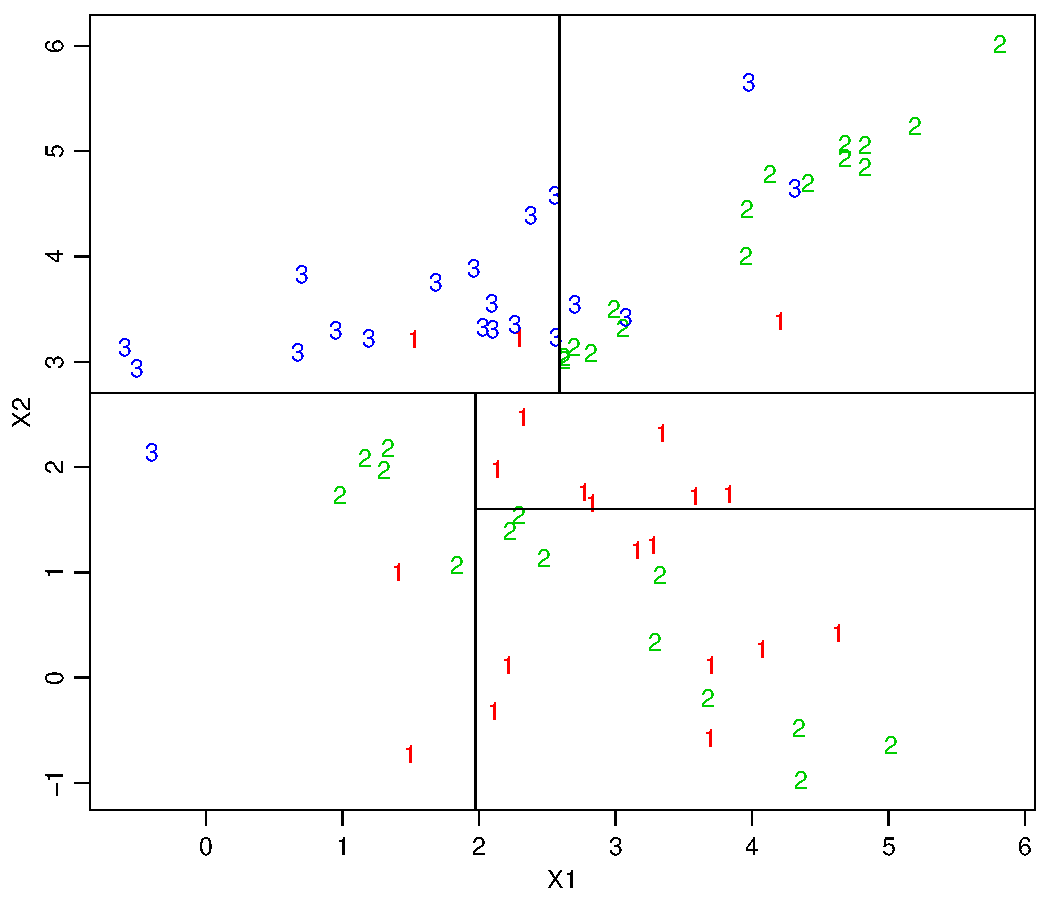
\includegraphics[width=\textwidth]{./figures/cartAreas1.pdf}
    \caption{Decisions displayed as boxes.}
    \label{fig:cartAreas1}
  \end{subfigure}%
  \quad
  \begin{subfigure}[b]{0.48\textwidth}
    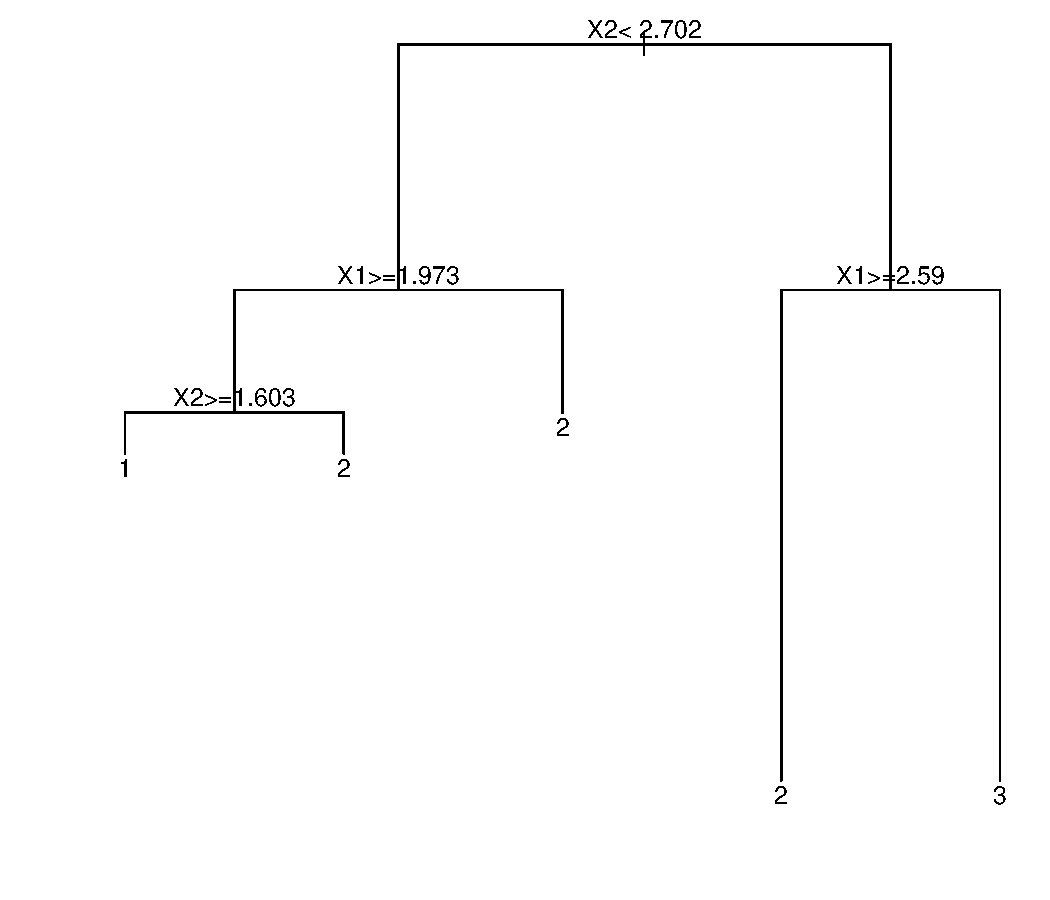
\includegraphics[width=\textwidth]{./figures/cartTree1.pdf}
    \caption{Decisions displayed as a tree.}
    \label{fig:cartTree1}
  \end{subfigure}
          %(or a blank line to force the subfigure onto a new line)
  \vspace{1\baselineskip}
  \caption{CART run on simulated data in two dimensions. }
  \label{fig:cart}
\end{figure}
%
\\
By now the intuition behind CART should be clear. What is not clear yet is how to grow the tree and how large the tree should be grown. As it is too computationally extensive to create an optimal tree, greedy algorithms for splitting are used for local splitting. A split needs to to be based on a criterion and one of the more common is the \textit{Gini index}
\begin{align}
  Q_m(T) &= \sum^{K}_{k=1} \hat{p}_{mk} (1 - \hat{p}_{mk}),  \\ 
  \label{eq:pmk} 
  \text{where}& \quad \hat{p}_{mk} = \frac{1}{N_m} \sum_{\mathbf{x}_i \in R_m} I\{y_i = k\}.
\end{align}
Here $T$ is the tree, $m$ is a node, $N_m$ is the number of data points in node $m$, $y_i$ is the class of point $i$ and $R_m$ is the region defined by the node.
$\hat{p}_{mk}$ is therefore the proportions of class $k$ in node $m$.
The Gini index gives a measure of \textit{node impurity}, as it increase with the diversity in the node. For nodes with only one class it is zero, and for homogeneous nodes it gets its maximum value. The greedy algorithm used by CART finds the split that gives the lowest total node impurity, and weight the nodes by the probability of sending a new point to that node.  \todo{confirm this} 
\\ \colorbox{yellow}{Comment how the length of a branch in Figure~\ref{fig:cartTree1} is proportional to the quality of the split.} \\ 
Consider the case where a split is performed on node $P$. By splitting on the variable $x_j$, let $R_L(j,s) = \{\mathbf{x} | x_j \leq s\}$ denote the region of the "left" split,  and $R_R(j,s) = \{\mathbf{x} | x_j > s\}$ denote the "right". To find the variable $x_j$ and split point $s$ that gives the lowest node impurity, one solve
\begin{align}
  \min_{j,s} \left\{ \frac{N_L}{N_P} Q_L(T)
  + \frac{N_R}{N_P} Q_R(T) \right\}.
\end{align}
Here $j$ and $s$ lies in $\hat{p}_{mk}$ in \eqref{eq:pmk}.
\todo{interpret gini indiex}
There are other measure of node impurity, like \textit{deviance} and \textit{misclassification error} used by CART. \colorbox{yellow}{These will be visited later}.\\
\colorbox{yellow}{Make sure that Gini is the original choice. If not, comment} \\
\\
It is now clear how to grow a tree, so the next step is to examine the tree size, to prevent over- or underfitting. The immediate idea one might get is to stop when the total Gini index change less than some threshold. This does not take into account that a seemingly worthless split might cause an excellent successive split. 
What CART does instead is to grow a large tree, and then \textit{prune} it back to find a local optimum. To prune a tree, is to collapse any number of internal nodes. 

Let $T_0$ denote the full tree and $T$ a subtree of $T_0$ that can be obtained by pruning. $|T|$ is the number of terminal nodes and $R_{\tau}$ is the region of of the terminal node $\tau$. The goal is to find the subtree $T_\alpha$ that minimizes some cost function $C_\alpha (T)$. It is usually the total terminal node impurity, but regularized by penalizing on the number of terminal nodes
\begin{align}
  C_\alpha (T) = \sum_{\tau = 1}^{|T|} Q_\tau (T) + \alpha |T|. 
\end{align}
This method is referred to as \textit{const-complexity pruning}.
Here the total Gini index can be used for $Q_\tau (T)$, but a more common choice is to use the \textit{misclassification rate} \todo{reference}
\begin{align}
  Q_\tau (T) =  \frac{1}{N_{\tau}} \sum_{\mathbf{x}_i \in R_{\tau}} I\{y_i \neq k(\tau)\},
\end{align}
where $k(\tau)$ is the predicted class in node $\tau$ (majority vote).
\\ \colorbox{yellow}{Is $y_i$ training data, test data, or CV?} \\
However, this is not an optimization problem easily solved by general solvers. Breiman et al. \cite{breiman} suggested a method called \textit{weakest link} pruning to find $T_\alpha$. They sequentially collapse the nodes that gives the smallest increase in $C_\alpha(T)$.
They proved that if continuing to collapse all the way back to a single node, $T_\alpha$ has to be in this sequence of subtrees.  \todo{Need to prove this?}. The only thing remaining then is to find the best $\alpha$. This is usually done by cross-validation, or, if the dataset is large, by misclassification error on a subset the training data, not used to build the tree. The latter is less computationally expensive, but can only be used on larger datasets. The final tree chosen is either the tree with the lowest MCE or the most parsimonious tree within 1 SD of that.
\\ \colorbox{yellow}{Not sure if $T_\alpha$ is found by $\min C_\alpha$ or CV over all sequential trees. Sources don't agree!}
\\ Pruning: \url{http://www.cbcb.umd.edu/~salzberg/docs/murthy_thesis/survey/node14.html}\\
\colorbox{yellow}{9.2.4 modstat Other issues: Categorical predictors} \\ \\
%
\colorbox{yellow}{Somethig on splitting on linear combinations of predictros. Good for prediction bad for interpreabillity}\\
\colorbox{yellow}{Do some simulations?}\\
\\\colorbox{yellow}{Mention other tree building algorithms? Shortly?}


